% =============================================================================
% Module 13: Gravitational Microlensing
% =============================================================================
% Source: Schneider, Kochanek & Wambsganss (2006), "Gravitational Lensing:
%         Strong, Weak and Micro", Part 4 (Microlensing, by J. Wambsganss),
%         Sects. 1, 2, 3, 4, 6, 7.
%         Paczynski (1986); Mao & Paczynski (1991); Paczynski (1998).
% Mathematica: ../Mathematica/13_Microlensing/
% =============================================================================

\chapter{Gravitational Microlensing}
\label{ch:microlensing}

\begin{quote}
\textit{``Of course, there is no great chance of observing this phenomenon
directly.''}
\hfill --- A. Einstein (1936), on star--star lensing
\end{quote}

\noindent
Einstein's pessimism was well founded for the technology of his day, but
spectacularly wrong for ours.  The images formed when one star lenses another
are split by only $\sim\!10^{-3}$~arcsec --- utterly unresolvable --- so the
individual images that dominated Modules~\ref{ch:lens_equation}
through~\ref{ch:elliptical_models} can never be seen.  What \emph{is}
observable is the \textbf{total magnification}, and because the lens, source,
and observer are all in relative motion, that magnification varies with time.
Monitoring millions of stars turns this tiny, transient brightening into one of
the most productive tools in modern astrophysics.  This is the regime of
\textbf{gravitational microlensing}, and it is the subject of this module,
which follows Part~4 of \citet{schneider_kochanek_wambsganss_2006}.

Microlensing recycles the physics we have already built --- it is the point-mass
lens of Module~\ref{ch:lens_equation} and the magnification formalism of
Module~\ref{ch:magnification}, read out in a new observational regime:
\begin{itemize}[nosep]
    \item the images are \textbf{unresolved}, so the observable is the
          time-variable \textbf{total magnification} $A(u)$, not image
          positions;
    \item the natural clock is the \textbf{Einstein-radius crossing time}
          $t_{\mathrm{E}}$, and the light curve has a universal, symmetric
          \textbf{Paczy\'nski} shape;
    \item ensembles of unseen lenses are characterized statistically through
          the \textbf{optical depth} $\tau$;
    \item small departures from the point-lens light curve reveal
          \textbf{binary companions and planets} (the caustics of
          Module~\ref{ch:elliptical_models} in miniature);
    \item the sub-milliarcsecond wobble of the light centroid
          (\textbf{astrometric microlensing}) and the micro-caustic networks
          that flicker across \textbf{multiply imaged quasars} (Modules~%
          \ref{ch:elliptical_models}--\ref{ch:galaxy_lensing}) extend the
          method to lens masses and quasar sizes.
\end{itemize}

\medskip
\noindent
\textbf{Companion Mathematica files:}
\begin{itemize}[nosep]
    \item \mathlink{13_Microlensing/microlensing.wl}{microlensing.wl}
          --- symbolic derivation of the point-lens magnification
          $A(u) = (u^2+2)/(u\sqrt{u^2+4})$ from the two images, its
          $u\to0$ and $u\to\infty$ limits, and the symmetry of the
          Paczy\'nski light curve about the peak; figures exported to
          \texttt{Figures/13\_Microlensing/}
    \item \mathlink{13_Microlensing/microlensing_explorer.nb}{microlensing\_explorer.nb}
          --- interactive notebook with \texttt{Manipulate} widgets for the
          light curve (vary $u_0$, $t_0$, $t_{\mathrm{E}}$) and for the
          binary-lens caustic topology (vary mass ratio $q$ and separation
          $d$)
\end{itemize}


% =====================================================================
\section{The Microlensing Regime}
\label{sec:micro_intro}

Consider a foreground star of mass $M$ at distance $\Dd$ lensing a background
star at distance $\Ds$.  The angular Einstein radius is
(eq.~\ref{eq:einstein_radius}, specialized to a point mass)
\begin{equation}
    \thetaE = \sqrt{\frac{4\Gnewton M}{\speedoflight^2}\,
    \frac{\Dds}{\Dd\,\Ds}} \,,
    \label{eq:micro_thetaE}
\end{equation}
which for stellar masses and kiloparsec distances evaluates to
$\thetaE \sim 10^{-3}$~arcsec (a \emph{milli}arcsecond --- hence
``\emph{micro}'' relative to the arcsecond image splittings of galaxy
lensing).  The two images produced by a point lens straddle the lens and are
separated by $\Delta\theta \approx 2\thetaE \sim$~mas, far below the
resolution of any conventional telescope.

The consequence is decisive: \textbf{individual image positions,
magnifications, and shapes are not measurable}.  All the information carried by
the image geometry in earlier modules is lost.  What survives is the
\emph{sum} of the image fluxes --- the total magnification --- which, thanks to
relative motion, sweeps out a light curve
\citep[Sect.~1]{schneider_kochanek_wambsganss_2006}.  The remainder of this
module is largely the study of that light curve and its perturbations.

\begin{remark}
Microlensing is defined by the \emph{observable}, not by the lens mass.  The
same point-mass physics describes a planet ($10^{-6}\,\Msun$) perturbing a
stellar event and a $30\,\Msun$ black hole in the Galactic halo.  What makes
all of these ``micro'' is that the image splitting is unresolved, so the total
magnification is the only handle.
\end{remark}


% =====================================================================
\section{Point-Lens Magnification}
\label{sec:point_lens_mag}

Scale all angles by $\thetaE$ and work with the dimensionless source position
$u \equiv \beta/\thetaE$ and image position $y \equiv \theta/\thetaE$.  The
point-mass lens equation (Module~\ref{ch:lens_equation}) reduces to the
one-dimensional form
\citep[eq.~1]{schneider_kochanek_wambsganss_2006}
\begin{equation}
    \boxed{\;u = y - \frac{1}{y}\;}
    \label{eq:micro_lens_eq}
\end{equation}
This is quadratic, $y^2 - u\,y - 1 = 0$, with the two roots
\begin{equation}
    y_\pm = \frac{1}{2}\left(u \pm \sqrt{u^2 + 4}\right) \,.
    \label{eq:micro_images}
\end{equation}
The two images always straddle the lens: $y_+ > 0$ lies on the same side as
the source (positive parity, brighter, always outside the Einstein ring),
while $y_- < 0$ lies on the opposite side (negative parity, fainter, inside
the ring).  Their separation is $|y_+ - y_-| = \sqrt{u^2 + 4}$.

\subsection{Magnification of Each Image}

For a circularly symmetric lens the signed magnification of an image at $y$ is
$\mu = [\,1 - y^{-4}\,]^{-1}$ (the product of the tangential and radial
eigenvalues, eq.~\ref{eq:eigenvalues_circular} evaluated for
$\alpha = 1/y$).  Substituting eq.~\eqref{eq:micro_images}
\citep[eq.~3]{schneider_kochanek_wambsganss_2006},
\begin{equation}
    \mu_\pm = \frac{1}{2}\left[\frac{u^2 + 2}{u\sqrt{u^2 + 4}} \pm 1\right] \,,
    \label{eq:micro_mu_pm}
\end{equation}
so that $\mu_+ > 0$, $\mu_- < 0$, and the images obey the sum rule
$\mu_+ + \mu_- = 1$.

\subsection{Total Magnification}

Because only the combined flux is observable, the relevant quantity is the
\textbf{total magnification} $A(u) = |\mu_+| + |\mu_-| = \mu_+ - \mu_-$:
\begin{equation}
    \boxed{\;A(u) = \frac{u^2 + 2}{u\,\sqrt{u^2 + 4}}\;}
    \label{eq:micro_A}
\end{equation}
This is the central formula of single-lens microlensing
\citep[eq.~4]{schneider_kochanek_wambsganss_2006}; the derivation by summing
the two image magnifications is verified symbolically in
\mathlink{13_Microlensing/microlensing.wl}{microlensing.wl}.  Its two limits
are physically important:
\begin{align}
    A(u) &\;\longrightarrow\; \frac{1}{u} \qquad (u \to 0) \,,
    \label{eq:micro_A_small} \\
    A(u) &\;\longrightarrow\; 1 \qquad\;\; (u \to \infty) \,.
    \label{eq:micro_A_large}
\end{align}
Close alignment ($u \to 0$) gives arbitrarily high magnification (formally
infinite for a point source at $u = 0$, where the images merge into an
Einstein ring), while a distant source ($u \gg 1$) is essentially unlensed.
At the fiducial separation $u = 1$ the magnification is
$A(1) = 3/\sqrt{5} \approx 1.34$, corresponding to a brightening of
$\Delta m = 2.5\log_{10}A \approx 0.32$~mag; the positive-parity image then
supplies $87\%$ of the total flux
\citep[Sect.~1.2]{schneider_kochanek_wambsganss_2006}.  The value $u = 1$ is
the conventional threshold defining a microlensing ``event''.

\begin{figure}[ht]
    \centering
    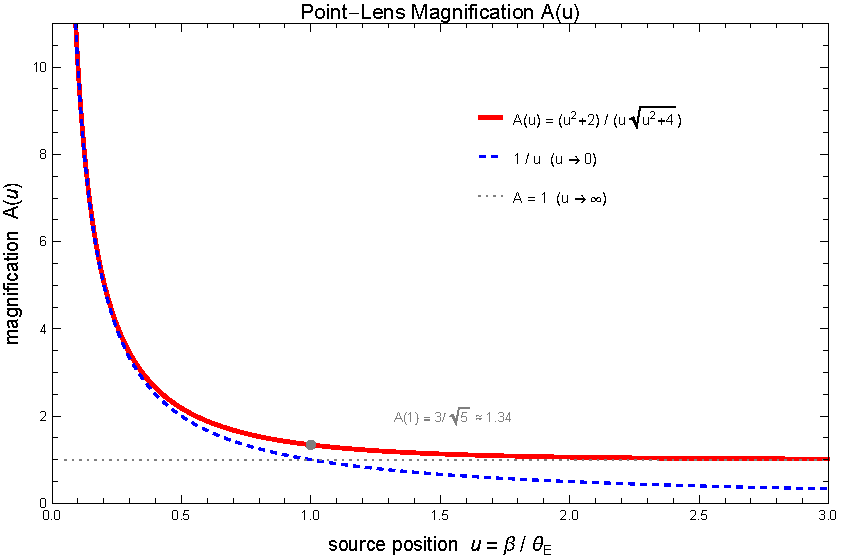
\includegraphics[width=0.72\textwidth]{../Figures/13_Microlensing/magnification_A_of_u.pdf}
    \caption{The point-lens total magnification $A(u)$
    (eq.~\ref{eq:micro_A}, red) as a function of the source--lens separation
    $u = \beta/\thetaE$.  The high-magnification asymptote $A \to 1/u$
    (blue dashed) and the unlensed limit $A \to 1$ (grey dotted) are shown for
    reference; the marked point is $A(1) = 3/\sqrt{5} \approx 1.34$.
    Generated by \texttt{microlensing.wl}.}
    \label{fig:micro_A}
\end{figure}


% =====================================================================
\section{The Light Curve and the Einstein Timescale}
\label{sec:lightcurve}

A microlensing event is a \emph{temporal} phenomenon.  Over the days-to-months
duration of an event the relative motion of lens and source is well
approximated as rectilinear, so the separation traces a straight line past the
lens.  Writing $t_0$ for the time of closest approach and $u_0$ for the
minimum (impact-parameter) separation, the source--lens separation is
\citep[eq.~8]{schneider_kochanek_wambsganss_2006}
\begin{equation}
    \boxed{\;u(t) = \sqrt{u_0^2 + \left(\frac{t - t_0}{t_{\mathrm{E}}}\right)^2}\;}
    \label{eq:micro_ut}
\end{equation}
where the \textbf{Einstein (crossing) timescale}
\begin{equation}
    t_{\mathrm{E}} \equiv \frac{\Dd\,\thetaE}{v_\perp}
    = \frac{\RE}{v_\perp}
    \label{eq:micro_tE}
\end{equation}
is the time for the lens to traverse one (physical) Einstein radius
$\RE = \Dd\,\thetaE$ at transverse speed $v_\perp$.  Substituting
eq.~\eqref{eq:micro_ut} into eq.~\eqref{eq:micro_A} gives the observed light
curve $F(t) = A(u(t))\,F_s$, where $F_s$ is the unlensed source flux.

\subsection{The Paczy\'nski Curve}

The resulting light curve --- the \textbf{Paczy\'nski curve}
\citep{paczynski_1986} --- is smooth, achromatic, and \emph{symmetric} about
$t_0$.  Symmetry follows immediately because $u(t)$ depends on time only
through $(t-t_0)^2$: $u(t_0+s) = u(t_0-s)$, hence
$A(u(t_0+s)) = A(u(t_0-s))$.  Since $A$ is a monotonically decreasing function
of $u$ (indeed $dA/du = -8/[u^2(u^2+4)^{3/2}] < 0$), the peak magnification
occurs at closest approach:
\begin{equation}
    A_{\max} = A(u_0) = \frac{u_0^2 + 2}{u_0\sqrt{u_0^2 + 4}}
    \;\approx\; \frac{1}{u_0}
    \quad (u_0 \ll 1) \,.
    \label{eq:micro_Amax}
\end{equation}
Both the symmetry and the identification $A_{\max} = A(u_0)$ are verified in
\mathlink{13_Microlensing/microlensing.wl}{microlensing.wl}.

The point-source, point-lens light curve is described by just four parameters:
the baseline flux $F_0$, the peak time $t_0$, the impact parameter $u_0$, and
the timescale $t_{\mathrm{E}}$.  Of these \emph{only $t_{\mathrm{E}}$ carries
physical information about the lens}, and it does so in the degenerate
combination $t_{\mathrm{E}} = \Dd\thetaE/v_\perp \propto \sqrt{M}$ that mixes
the lens mass $M$, distance $\Dd$, and transverse velocity $v_\perp$
\citep[Sect.~1.2]{schneider_kochanek_wambsganss_2006}.  Breaking this
degeneracy --- to weigh the lens --- requires extra information: finite-source
effects, parallax, or the astrometric shift of \S\ref{sec:astrometric}.

\begin{example}
\textbf{A typical Galactic event.}
For a lens of $M = 0.3\,\Msun$ halfway to a bulge source
($\Dd = 4$~kpc, $\Ds = 8$~kpc) moving at $v_\perp = 200$~km\,s$^{-1}$,
eqs.~\eqref{eq:micro_thetaE} and~\eqref{eq:micro_tE} give
$\thetaE \approx 0.55$~mas, $\RE \approx 2.2$~AU, and
$t_{\mathrm{E}} \approx 19$~days --- of order weeks, as observed.  The
numbers are computed in
\solnlink{13_Microlensing/problems\_13.wl}{problems\_13.wl}.
\end{example}

\begin{figure}[ht]
    \centering
    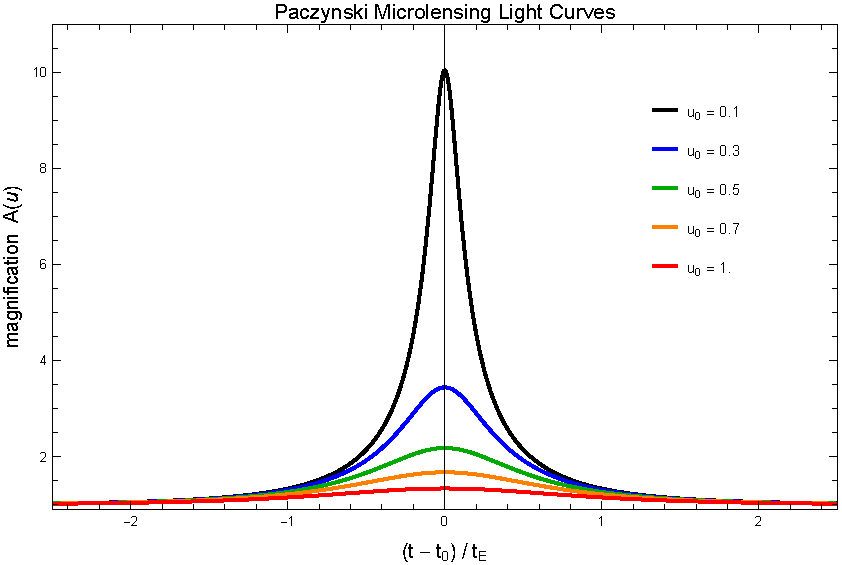
\includegraphics[width=0.72\textwidth]{../Figures/13_Microlensing/paczynski_lightcurves.pdf}
    \caption{Paczy\'nski microlensing light curves (eq.~\ref{eq:micro_ut}
    substituted into eq.~\ref{eq:micro_A}) for minimum impact parameters
    $u_0 = 0.1, 0.3, 0.5, 0.7, 1.0$ (top to bottom).  Time is in units of the
    Einstein timescale $t_{\mathrm{E}}$; every curve is symmetric about the
    peak at $(t-t_0)/t_{\mathrm{E}} = 0$, and the smaller the impact parameter
    the higher and narrower the peak ($A_{\max} \approx 1/u_0$).
    Generated by \texttt{microlensing.wl}.}
    \label{fig:micro_lightcurves}
\end{figure}


% =====================================================================
\section{Optical Depth to Microlensing}
\label{sec:optical_depth}

A single event is rare, so microlensing is inherently a statistical enterprise:
one monitors millions of stars to catch a handful of events.  The relevant
statistic is the \textbf{optical depth} $\tau$, the probability that a random
source lies within one Einstein radius of some lens at a given instant ---
equivalently, the fraction of the sky covered by the Einstein disks of all the
lenses \citep[Sect.~1.4]{schneider_kochanek_wambsganss_2006}.

For lenses distributed with mass density $\rho(\Dd)$ along the line of sight,
\citet{paczynski_1986} showed
\begin{equation}
    \boxed{\;\tau = \int_0^{\Ds}
    \frac{4\pi\Gnewton}{\speedoflight^2}\,
    \frac{\Dd\,\Dds}{\Ds}\,\rho(\Dd)\,d\Dd\;}
    \label{eq:micro_tau}
\end{equation}
Remarkably, $\tau$ is \emph{independent of the individual lens masses}: it
depends only on the total mass density, because the Einstein area
$\pi\thetaE^2 \propto M$ while the number density $\propto 1/M$, and the two
cancel.  The equivalence of ``fraction of sky in Einstein disks'' and
$\Sigma/\Sigmacr$ for a thin lens screen is verified in
\solnlink{13_Microlensing/problems\_13.wl}{problems\_13.wl}.

\subsection{The Dark-Matter Test Toward the Magellanic Clouds}

Paczy\'nski's motivation was profound: if the dark halo of the Milky Way were
made of compact objects (MACHOs --- MAssive Compact Halo Objects), they would
microlens background stars in the Large and Small Magellanic Clouds
(LMC/SMC).  For a standard isothermal halo he predicted
\begin{equation}
    \tau_{\mathrm{halo}} \sim 5 \times 10^{-7} \,,
    \label{eq:micro_tau_halo}
\end{equation}
so roughly one star in two million is measurably lensed at any time --- a small
but tractable number given large CCD surveys.  The MACHO, EROS, and OGLE
collaborations carried out the experiment through the 1990s and 2000s.  Their
verdict: the observed rate toward the LMC,
$\tau_{\mathrm{LMC}} \approx 1.2^{+0.4}_{-0.3} \times 10^{-7}$ (MACHO), is far
too low for compact objects to constitute the entire halo.  MACHOs in the
mass range $\sim\!10^{-7}$ to $1\,\Msun$ contribute less than about $25\%$ of
the halo, and the surviving events are consistent with ordinary stars in the
disk or within the Clouds themselves
\citep[Sect.~3.5]{schneider_kochanek_wambsganss_2006}.  This is a landmark
\emph{null} result: it decisively ruled out baryonic compact objects as the
dominant dark matter.

\subsection{Toward the Galactic Bulge}

Monitoring the crowded Galactic bulge yields events with near certainty and a
much higher optical depth,
$\tau_{\mathrm{bulge}} \approx (0.9\text{--}3) \times 10^{-6}$, tracing the
stellar bar along the line of sight
\citep[Sect.~3.6]{schneider_kochanek_wambsganss_2006}.  The bulge is now the
principal hunting ground for the planetary events of the next section.


% =====================================================================
\section{Binary and Planetary Microlensing}
\label{sec:binary_planet}

A single point lens has only a degenerate point caustic at $u=0$.  As soon as
a \emph{second} mass is added, the lens becomes non-axisymmetric and develops
\textbf{extended caustics} in the source plane --- exactly the fold-and-cusp
curves of Module~\ref{ch:elliptical_models}, now realized at stellar scales.
For a binary lens the deflection is the sum of two point-mass terms
\citep[eq.~14]{schneider_kochanek_wambsganss_2006},
\begin{equation}
    \vecalpha(\vectheta) = \frac{4\Gnewton}{\speedoflight^2}
    \left[
    \frac{M_A(\vectheta - \vectheta_A)}{|\vectheta - \vectheta_A|^2}
    + \frac{M_B(\vectheta - \vectheta_B)}{|\vectheta - \vectheta_B|^2}
    \right] \,,
    \label{eq:micro_binary_alpha}
\end{equation}
and the system is described by three new parameters: the mass ratio
$q = M_B/M_A$, the projected separation $d$ (in units of $\thetaE$ of the total
mass), and the angle $\phi$ of the source trajectory relative to the binary
axis.  The caustic topology changes qualitatively with $d$: widely separated
lenses have two small asteroid-shaped caustics; near $d \approx 1$ these merge
through an intermediate six-cusp caustic; and at $d = 8^{-1/2} \approx 0.354$
the caustic splits into a central four-cusp plus two triangular caustics
\citep[Sect.~2.1]{schneider_kochanek_wambsganss_2006, petters_singularity_2001}.

\subsection{Caustic Crossings}

The observational signature is dramatic.  When the source \emph{crosses} a
caustic, a pair of highly magnified images is created or destroyed, and because
these images dominate the (unresolved) total flux, the light curve shows a
sharp spike.  A point source would formally be infinitely magnified at the
caustic; the finite spike height instead \emph{measures the source size},
since the magnification is smeared over the time
$t_{\mathrm{cross}} = R_{\mathrm{source}}/v_\perp$ it takes the source to cross
its own diameter.  Caustic-crossing binaries thus break the point-source
approximation in a useful way, occasionally even resolving the stellar surface
brightness profile.

\subsection{Detecting Planets}

\citet{mao_paczynski_1991} first showed that a planetary companion to the lens
star produces the same kind of short, low-amplitude deviation on top of an
otherwise ordinary stellar light curve, and estimated that of order $10\%$ of
events should show a detectable binary signature.  A planet of mass ratio
$q = M_{\mathrm{planet}}/M_\star$ generates a small caustic whose perturbation
is strongest when the projected separation lies in the \textbf{lensing zone}
$0.6 \lesssim d/\thetaE \lesssim 1.6$, where the planetary caustic falls near
the Einstein ring of the host star
\citep[Sect.~4.1]{schneider_kochanek_wambsganss_2006}.  By a fortunate
coincidence this angular range corresponds to physical separations of order
$1$~AU for typical Galactic lenses --- overlapping the habitable zone.  The
planetary deviation is brief (hours to a day) and of small amplitude (a few
percent), so dense, continuous monitoring of ongoing stellar events is
required.  Microlensing is uniquely sensitive to \emph{cool, low-mass planets
at $\sim\!1$--$10$~AU} around distant ($\sim$~kpc) stars, a region of parameter
space complementary to radial-velocity and transit surveys.  Its cost is that
each event is a unique, non-repeatable alignment, and only the mass \emph{ratio}
$q$ (not the planet mass directly) is measured from the light curve alone.


% =====================================================================
\section{Astrometric Microlensing}
\label{sec:astrometric}

Although the two images cannot be resolved, their flux-weighted mean
position --- the \textbf{light centroid} --- is displaced from the true source
position, and that displacement can in principle be measured to
sub-milliarcsecond precision.  This is \textbf{astrometric microlensing}
\citep[Sect.~6]{schneider_kochanek_wambsganss_2006}.  Combining the image
positions~\eqref{eq:micro_images} with their
magnifications~\eqref{eq:micro_mu_pm}, the centroid shift relative to the
source is
\begin{equation}
    \delta(u) = \frac{u}{u^2 + 2}\,\thetaE \,.
    \label{eq:micro_centroid}
\end{equation}
Unlike the photometric magnification, the centroid shift \emph{vanishes} both
at perfect alignment ($u\to0$) and at large separation ($u\to\infty$); it is
maximized in between.  Setting $d\delta/du = 0$ gives
\begin{equation}
    \boxed{\;\delta_{\max} = \frac{1}{2\sqrt{2}}\,\thetaE
    = 8^{-1/2}\,\thetaE \approx 0.354\,\thetaE
    \quad\text{at}\quad u = \sqrt{2}\;}
    \label{eq:micro_centroid_max}
\end{equation}
\citep[eq.~22]{schneider_kochanek_wambsganss_2006}, a result due to
\citet{paczynski_1998}; both the location $u = \sqrt{2}$ and the peak value are
verified in \mathlink{13_Microlensing/microlensing.wl}{microlensing.wl}.

The astrometric signal is valuable because the centroid traces an ellipse
whose \emph{angular} size is set directly by $\thetaE \propto \sqrt{M}$.
Measuring it therefore yields $\thetaE$, and combined with a parallax
measurement it breaks the mass--distance--velocity degeneracy entirely,
delivering the lens mass:
\begin{equation}
    M = 0.123\,\Msun\;
    \frac{\thetaE^2}{\pi_{\mathrm{ds}}}
    \label{eq:micro_astro_mass}
\end{equation}
with $\thetaE$ and the lens--source relative parallax $\pi_{\mathrm{ds}}$ in
milliarcseconds
\citep[eq.~25]{schneider_kochanek_wambsganss_2006}.  The centroid shift is
tens to hundreds of micro-arcseconds --- beyond ground-based astrometry of the
2000s, but squarely within reach of space astrometry (the numerical
coefficient is checked in
\solnlink{13_Microlensing/problems\_13.wl}{problems\_13.wl}).


% =====================================================================
\section{Quasar Microlensing}
\label{sec:quasar}

Microlensing is not confined to the Milky Way.  When a distant quasar is
multiply imaged by a foreground galaxy (Modules~\ref{ch:elliptical_models}
and~\ref{ch:galaxy_lensing}), the individual \emph{stars} of that galaxy
microlens each macro-image.  This is \textbf{quasar microlensing}
\citep[Sect.~7]{schneider_kochanek_wambsganss_2006}.  The key contrast with
Galactic microlensing is that at the position of a macro-image the stellar
convergence is of order unity, $\kappab \sim 1$, so at any instant a
\emph{whole ensemble} of stars lenses the source coherently, producing an
intricate \textbf{network of micro-caustics} in the source plane rather than a
single isolated event.

The relevant scales, for typical lens and source redshifts
$z_d \approx 0.5$, $z_s \approx 2$, are the Einstein radius projected into the
quasar plane and its crossing time
\citep[Sect.~7.1]{schneider_kochanek_wambsganss_2006}:
\begin{align}
    r_{\mathrm{E}} &\approx 4 \times 10^{16}\,
    \left(\frac{M}{\Msun}\right)^{1/2}\,\text{cm} \,,
    \label{eq:micro_qso_rE} \\
    t_{\mathrm{E}} &\approx 15\,
    \left(\frac{M}{\Msun}\right)^{1/2}
    \left(\frac{v_\perp}{600~\text{km s}^{-1}}\right)^{-1}\,\text{yr} \,.
    \label{eq:micro_qso_tE}
\end{align}
The full Einstein-crossing time is discouragingly long, but the observable
fluctuations are governed instead by the much shorter \emph{caustic}-crossing
time $t_{\mathrm{cross}} = R_{\mathrm{source}}/v_\perp \approx 4\,(R_{15})\,
(v_\perp/600~\text{km s}^{-1})^{-1}$~months, where the quasar continuum size
$R_{15}$ is in units of $10^{15}$~cm.  The scale estimates and the
$\propto\sqrt{M}$ mass scaling are checked in
\solnlink{13_Microlensing/problems\_13.wl}{problems\_13.wl}.

The great power of quasar microlensing is that $t_{\mathrm{cross}}$ ---
and hence the sharpness of the microlensing fluctuations --- is set by the
\emph{source size}: a compact continuum-emitting region crosses caustics
cleanly and flickers strongly, whereas a large emission region washes the
peaks out.  Monitoring the uncorrelated (non-time-delayed) variability between
the macro-images therefore constrains the \textbf{quasar accretion-disk size},
independently of the time-delay cosmography of Module~\ref{ch:galaxy_lensing}.
The classic laboratory is the ``Einstein Cross'' Q2237$+$0305, whose four
images vary independently by up to $\sim\!1$~mag; the fits imply a continuum
region of order $10^{14}$~cm
\citep[Sect.~7.3]{schneider_kochanek_wambsganss_2006}.  Quasar microlensing
also probes the fraction of the lens-galaxy mass in compact objects versus
smooth dark matter, complementing the halo constraints of
\S\ref{sec:optical_depth}.


% =====================================================================
\section{Summary}
\label{sec:micro_summary}

\begin{itemize}
    \item In the \textbf{microlensing regime} the two point-lens images are
          split by only $\sim$~mas and are unresolved, so the sole observable
          is the time-variable \textbf{total magnification}
          $A(u) = (u^2+2)/(u\sqrt{u^2+4})$, with
          $u = \beta/\thetaE$.

    \item $A(u) \to 1/u$ at high magnification ($u\to0$) and $A(u)\to1$ at
          large separation ($u\to\infty$); the event threshold is $u = 1$,
          where $A = 3/\sqrt{5} \approx 1.34$.

    \item Relative motion turns $A$ into the symmetric \textbf{Paczy\'nski
          light curve} $A(u(t))$ with
          $u(t) = \sqrt{u_0^2 + (t-t_0)^2/t_{\mathrm{E}}^2}$, peaking at
          $A_{\max} = A(u_0)$.  Only the \textbf{Einstein timescale}
          $t_{\mathrm{E}} = \Dd\thetaE/v_\perp \propto \sqrt{M}$ carries
          physical information, in a mass--distance--velocity degenerate
          combination.

    \item The \textbf{optical depth}
          $\tau = \int (4\pi\Gnewton/\speedoflight^2)(\Dd\Dds/\Ds)\rho\,d\Dd$
          is mass-independent.  Toward the LMC the measured
          $\tau \approx 1.2\times10^{-7}$ rules out MACHOs as the dominant
          dark matter ($\lesssim 25\%$ of the halo); toward the bulge
          $\tau \sim 10^{-6}$.

    \item \textbf{Binary and planetary} lenses add extended caustics; caustic
          crossings give sharp, source-size-dependent spikes, and a planet in
          the lensing zone $0.6 \lesssim d/\thetaE \lesssim 1.6$ produces a
          brief low-amplitude deviation revealing the mass ratio $q$.

    \item \textbf{Astrometric} microlensing measures the light-centroid shift,
          peaking at $\delta_{\max} = 8^{-1/2}\thetaE$ for $u = \sqrt2$; with a
          parallax it yields the lens mass.

    \item \textbf{Quasar} microlensing ($\kappab\sim1$, micro-caustic
          networks) constrains quasar accretion-disk sizes and the compact-object
          content of lens galaxies.
\end{itemize}


% =====================================================================
\section{Problems}
\label{sec:micro_problems}

\begin{exercise}
\label{ex:micro_magnification}
\textbf{(Total magnification and its limits.)}
Work in Einstein units, $u = \beta/\thetaE$, $y = \theta/\thetaE$.
\begin{enumerate}[label=(\alph*)]
    \item Solve the point-lens equation $u = y - 1/y$ for the two image
          positions $y_\pm$ and verify the separation
          $|y_+ - y_-| = \sqrt{u^2+4}$.
    \item Using $\mu = [1 - y^{-4}]^{-1}$, show that the total magnification
          is $A(u) = |\mu_+| + |\mu_-| = (u^2+2)/(u\sqrt{u^2+4})$.
    \item Verify the limits $A(u)\to1/u$ as $u\to0$ and $A(u)\to1$ as
          $u\to\infty$.
    \item Compute the peak brightening $\Delta m$ (in magnitudes) for an event
          with impact parameter $u_0 = 1$.
\end{enumerate}
Verify with
\solnlink{13_Microlensing/problems\_13.wl}{problems\_13.wl}.
\end{exercise}

\begin{exercise}
\label{ex:micro_timescale}
\textbf{(Einstein radius and timescale.)}
\begin{enumerate}[label=(\alph*)]
    \item For a lens of $M = 0.3\,\Msun$ at $\Dd = 4$~kpc lensing a bulge
          source at $\Ds = 8$~kpc, compute the angular Einstein radius
          $\thetaE$ (in mas) and the physical Einstein radius $\RE$ (in AU).
    \item For a transverse speed $v_\perp = 200$~km\,s$^{-1}$, compute the
          Einstein timescale $t_{\mathrm{E}}$ in days.  Comment on why
          Galactic events last of order weeks.
    \item Show that at fixed geometry and velocity
          $t_{\mathrm{E}} \propto \sqrt{M}$, and hence that the light curve
          alone cannot separate $M$, $\Dd$, and $v_\perp$.  What additional
          measurements break this degeneracy?
\end{enumerate}
Verify with
\solnlink{13_Microlensing/problems\_13.wl}{problems\_13.wl}.
\end{exercise}

\begin{exercise}
\label{ex:micro_optical_depth}
\textbf{(Optical depth and the MACHO test.)}
\begin{enumerate}[label=(\alph*)]
    \item Explain physically why the optical depth $\tau$
          (eq.~\ref{eq:micro_tau}) is independent of the individual lens
          masses.  \textit{Hint:} how do the Einstein area and the number
          density each scale with $M$?
    \item For a thin lens screen of surface mass density $\Sigma$, show that
          the fraction of sky covered by Einstein disks equals
          $\Sigma/\Sigmacr$.
    \item Given the Paczy\'nski halo value $\tau \sim 5\times10^{-7}$,
          how many stars must be monitored to expect of order one lensed star
          at any instant?
    \item The measured LMC value is $\tau \approx 1.2\times10^{-7}$, well
          below the prediction for a fully compact halo.  What does this imply
          about MACHOs as a dark-matter candidate?
\end{enumerate}
Verify with
\solnlink{13_Microlensing/problems\_13.wl}{problems\_13.wl}.
\end{exercise}

\begin{exercise}
\label{ex:micro_peak}
\textbf{(Peak magnification and event width.)}
\begin{enumerate}[label=(\alph*)]
    \item An event reaches peak magnification $A_{\max} = 5$.  Invert
          eq.~\eqref{eq:micro_Amax} to find the impact parameter $u_0$.
    \item Show that the high-magnification approximation
          $A_{\max}\approx1/u_0$ is accurate to better than $1\%$ for
          $u_0 = 0.05$.
    \item Show that the source reaches the event threshold $u = 1$ (where
          $A = 3/\sqrt5$) at times $|t - t_0| = t_{\mathrm{E}}\sqrt{1-u_0^2}$,
          for $u_0 < 1$.
\end{enumerate}
Verify with
\solnlink{13_Microlensing/problems\_13.wl}{problems\_13.wl}.
\end{exercise}

\begin{exercise}
\label{ex:micro_astrometric}
\textbf{(Astrometric centroid shift.)}
The light centroid of a point-lens event is displaced from the source by
$\delta(u) = u\,\thetaE/(u^2+2)$.
\begin{enumerate}[label=(\alph*)]
    \item Show that $\delta(u)$ is maximized at $u = \sqrt2$.
    \item Evaluate the maximum shift and show it equals
          $\delta_{\max} = 8^{-1/2}\,\thetaE \approx 0.354\,\thetaE$.
    \item Explain why the astrometric signal breaks the mass--distance
          degeneracy that the photometric light curve cannot, and identify
          the coefficient in the mass relation
          $M = 0.123\,\Msun\,\thetaE^2/\pi_{\mathrm{ds}}$ (with angles in mas).
\end{enumerate}
Verify with
\solnlink{13_Microlensing/problems\_13.wl}{problems\_13.wl}.
\end{exercise}

\begin{exercise}
\label{ex:micro_quasar}
\textbf{(Quasar microlensing scales.)}
\begin{enumerate}[label=(\alph*)]
    \item For a quasar at $z_s \approx 2$ microlensed by stars in a galaxy at
          $z_d \approx 0.5$, estimate the Einstein radius projected into the
          source plane for a solar-mass star, and show it is of order
          $10^{16}$~cm.
    \item Show $r_{\mathrm{E}} \propto \sqrt{M}$.
    \item Estimate the caustic-crossing time
          $t_{\mathrm{cross}} = R_{\mathrm{source}}/v_\perp$ for a continuum
          region of $R = 10^{15}$~cm and $v_\perp = 600$~km\,s$^{-1}$, and
          explain why this (not $t_{\mathrm{E}}$) sets the observable
          variability timescale.
    \item Why does the condition $\kappab \sim 1$ at a quasar macro-image mean
          that microlensing acts as a \emph{network} of caustics rather than
          isolated events?
\end{enumerate}
Verify with
\solnlink{13_Microlensing/problems\_13.wl}{problems\_13.wl}.
\end{exercise}
